\documentclass[margin=10pt]{standalone}

\usepackage{tikz}

\usetikzlibrary{decorations.pathreplacing,arrows,shapes,positioning,shadows,calc}

\begin{document}

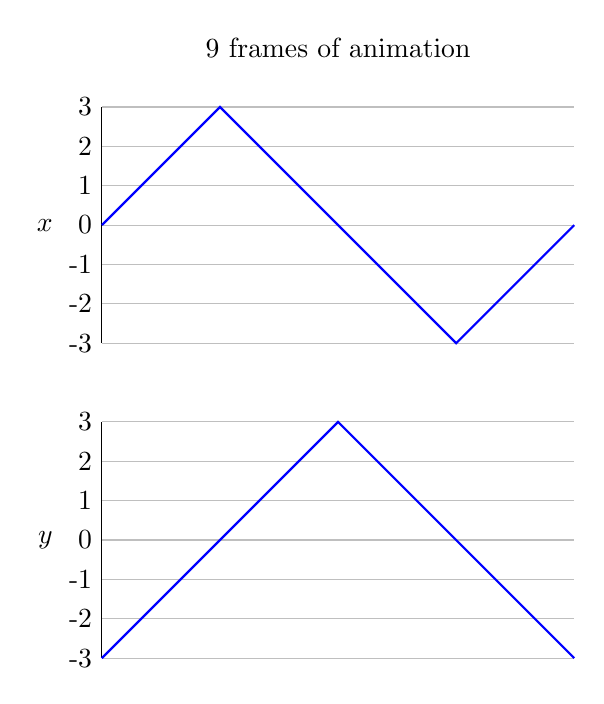
\begin{tikzpicture}[scale=0.5]
%	\draw (0,0) rectangle (10,7);
	\draw (0,0) node[anchor=north] {9 frames of animation};
	
	\begin{scope}[shift={(-6,-5)}]
		\draw (0,-3) -- (0,3);
		
		\draw (-1,0) node[anchor=east] {$x$};

		\draw (0,-3) node[anchor=east] {-3};
		\draw (0,-2) node[anchor=east] {-2};
		\draw (0,-1) node[anchor=east] {-1};
		\draw (0,0) node[anchor=east] {0};
		\draw (0,1) node[anchor=east] {1};
		\draw (0,2) node[anchor=east] {2};
		\draw (0,3) node[anchor=east] {3};
		
		\draw[lightgray] (0,-3) -- ++ (12,0);
		\draw[lightgray] (0,-2) -- ++ (12,0);
		\draw[lightgray] (0,-1) -- ++ (12,0);
		\draw[lightgray] (0,0) -- ++ (12,0);
		\draw[lightgray] (0,1) -- ++ (12,0);
		\draw[lightgray] (0,2) -- ++ (12,0);
		\draw[lightgray] (0,3) -- ++ (12,0);
		
		\draw[thick,blue] (0,0) -- (3,3) -- (9,-3) -- (12,0);
	\end{scope}

	\begin{scope}[shift={(-6,-13)}]
		\draw (0,-3) -- (0,3);
		
		\draw (-1,0) node[anchor=east] {$y$};

		\draw (0,-3) node[anchor=east] {-3};
		\draw (0,-2) node[anchor=east] {-2};
		\draw (0,-1) node[anchor=east] {-1};
		\draw (0,0) node[anchor=east] {0};
		\draw (0,1) node[anchor=east] {1};
		\draw (0,2) node[anchor=east] {2};
		\draw (0,3) node[anchor=east] {3};
		
		\draw[lightgray] (0,-3) -- ++ (12,0);
		\draw[lightgray] (0,-2) -- ++ (12,0);
		\draw[lightgray] (0,-1) -- ++ (12,0);
		\draw[lightgray] (0,0) -- ++ (12,0);
		\draw[lightgray] (0,1) -- ++ (12,0);
		\draw[lightgray] (0,2) -- ++ (12,0);
		\draw[lightgray] (0,3) -- ++ (12,0);
		
		\draw[thick,blue] (0,-3) -- (6,3) -- (12,-3);
	\end{scope}
\end{tikzpicture}

\end{document}